%==================== PARTE C: QUESTÕES 3 E 4 (PREPARAÇÃO EXPERIMENTAL) ====================
\section{Questões 3 e 4: preparação experimental (a realizar)}\label{q34}
Esta parte segue o \textbf{mesmo padrão} dos itens da Questão 1 (Seções~\ref{expq11} a \ref{expq13}): objetivo e fundamentos, como digitar a sintonia no programa do PLC, procedimento, \textbf{previsão da simulação ideal} (planta completa, sem ruído do ADC, com os limites do SC do programa), planilha de resultados a preencher, roteiro de interpretação e riscos. Os ensaios dos itens 3.1, 4.1 e 4.2 \textbf{serão realizados depois}; as caixas amarelas e as tabelas ``Experimento'' ficam em branco para serem preenchidas. A teoria e os cálculos das sintonias estão nas Seções~\ref{it31} e \ref{it41}; o item 4.2 (I\_PD) é desenvolvido aqui.

\subsection{Roteiro comum aos ensaios}\label{roteirocomum}
\begin{enumerate}
\item \textbf{Programa.} Usar o \texttt{Prova2\_corrigido.st} (projeto corrigido, Seção~\ref{progcorr}) \emph{ou}, se for repetir exatamente os ensaios da Questão 1, o \texttt{Prova2.st}. Com a derivada sem filtro do programa original, os ganhos $k_d$ destes itens ($71{,}6$ e $197{,}3$) geram pulsos de 140 e 385 pontos por LSB da VP (Seção~\ref{expruido}), e o SO fica saturado em 10 e 100\,\%; os resultados experimentais seriam distorcidos.
\item \textbf{Condição inicial (manual).} $SO_0=\dfrac{SP_0+0{,}262}{0{,}3963}$ (inversa do ajuste da Seção~\ref{expplanta}); esperar $\ge8$ min ($\ge7\tau_1$) até a VP estabilizar em $SP_0$. Em manual o programa faz $SP=VP$ (VP-tracking), então o SP já fica igual à VP no instante de fechar a malha.
\item \textbf{Fechar a malha} (\texttt{MF := 1}) com $SP=VP$; aguardar 50 s; \textbf{aplicar o degrau de SP}; gravar até a VP assentar (400--700 s).
\item \textbf{Registro:} ScadaBR a 1 s, pontos SO, SP, VP, VP1, VP2. Anotar a versão do programa, os valores digitados e os instantes das ações.
\item \textbf{Comparação:} \texttt{python3 codigos/simula\_bancada.py comparar ARQUIVO.csv --inicio <t\_fechamento> --kp .. --ti .. --td .. --sat --aw clamp} (RMS e erro máximo de VP e de SC, com a mediana móvel do SO). A tabela ``Experimento'' de cada item usa as mesmas métricas da Questão 1: sobressinal, $t_{63,2}$, tempo de acomodação ($\pm2\,\%$ do degrau), pico e valor final do SC, RMS e erro máximo da VP.
\end{enumerate}
\begin{just}\textbf{Por que estas escolhas.} A condição inicial longa evita que o transitório do circuito contamine o degrau (o polo dominante é $\tau_1=68{,}7$ s). O degrau é pequeno porque o SC tem limites $[10;100]\,\%$ e o salto proporcional $K_p\Delta SP$ é grande nestas sintonias. O $SC_0$ inclui o offset ($-0{,}262$) medido no dia dos ensaios.\end{just}

%------------------------------------------------------------------
\section{Item 3.1 (Questão 3): integral do erro mínimo (seção 7-2.3)}\label{q31exp}
\subsection{Objetivo e fundamentos}
Verificar experimentalmente a sintonia do PID pelas correlações de IAE mínimo para \emph{ponto fixo} (Tabela 7-2.3, Rovira), calculadas na Seção~\ref{it31} com $K=0{,}3918$, $\tau=78{,}03$ s, $t_0=25{,}92$ s ($r=t_0/\tau=0{,}3322$):
\[
K_c=\frac{1{,}086}{K}r^{-0{,}869}=7{,}222,\qquad\tau_I=\frac{\tau}{0{,}740-0{,}130r}=111{,}98\ \mathrm{s},\qquad\tau_D=0{,}348\,\tau\,r^{0{,}914}=9{,}92\ \mathrm{s}.
\]
Estas tabelas já dão o PID na forma \emph{ideal} (paralela), então $K_p=K_c$, $K_i=K_c/\tau_I=0{,}06449$ e $K_d=K_c\tau_D=71{,}63$ (sem conversão série$\to$ideal). A sintonia minimiza $\int|e|\,dt$ para um degrau de SP, \emph{sem penalizar o esforço de controle}: espera-se resposta rápida, algum sobressinal e SC com pico grande.
\subsection{Como digitar no programa}
\begin{center}\small\begin{tabular}{lcccc}\toprule \texttt{kp} & \texttt{ki} & \texttt{kd} & \texttt{alfa} & degrau de SP\\\midrule 7.222 & 0.06449 & 71.63 & 1.0 (PI\_D) & $20\to25\,\%$\\\bottomrule\end{tabular}\end{center}
$SO_0=(20+0{,}262)/0{,}3963=51{,}1\,\%$; $SO$ final esperado $=(25+0{,}262)/0{,}3963=63{,}7\,\%$.
\subsection{Previsão da simulação ideal}
\begin{figure}[H]\centering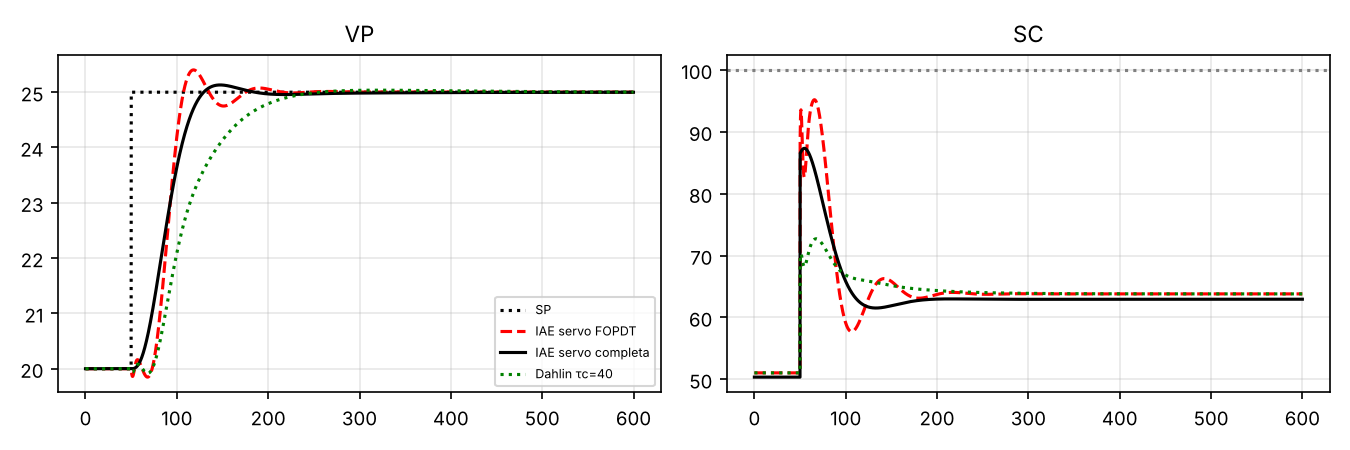
\includegraphics[width=.98\textwidth]{figs/i31.png}\caption{Item 3.1, simulação ideal: IAE ponto fixo (FOPDT tracejado vermelho; FT completa preto) e Dahlin $\tau_c=40$ s do item 1.1 (verde pontilhado), degrau $20\to25\,\%$.}\end{figure}
\begin{center}\small
\begin{tabular}{lccc}\toprule Métrica & Ideal FOPDT & Ideal FT completa & \textbf{Experimento}\\\midrule
Sobressinal [\%] & 8,1 & 2,6 & \underline{\hspace{1.6cm}}\\
$t_{63,2}$ [s] & 44 & 44 & \underline{\hspace{1.6cm}}\\
Tempo de acomodação ($\pm2\,\%$) [s] & 117 & 110 & \underline{\hspace{1.6cm}}\\
Pico do SC [\%] & 95 & 87 & \underline{\hspace{1.6cm}}\\
SC final [\%] & 63,8 & 62,9 & \underline{\hspace{1.6cm}}\ (previsto 63,7)\\
Salto do SC em $t=50$ s [pontos] & \multicolumn{2}{c}{$K_p\Delta SP=7{,}222\cdot5=36{,}1$} & \underline{\hspace{1.6cm}}\\
Erro VP: RMS / máx.\ [\%] & --- & --- & \underline{\hspace{1.6cm}}\\\bottomrule\end{tabular}\end{center}
Margens da malha aberta com esta sintonia: FOPDT $GM=1{,}9$, $PM=64^\circ$; FT completa $GM=32{,}0$, $PM=71^\circ$. Para comparação, a sintonia de \emph{distúrbio} (Tabela 7-2.2, $K_p=10{,}1$) aplicada a um degrau de SP daria sobressinal de 84\,\% (FOPDT) e 42\,\% (completa).
\subsection{Roteiro de interpretação (o que escrever)}
\begin{itemize}
\item \textbf{Salto de SC:} confira $\Delta SC(0^+)=K_p\Delta SP=36{,}1$ (como na Q11: previsto 36,9, medido 37,0). Isso confirma $K_p$ digitado.
\item \textbf{Mais rápida que o Dahlin do 1.1:} $t_{63}\approx44$ s contra $\approx70$ s; o custo é o sobressinal (2,6\,\% a 8,1\,\%) e o pico de SC ($\approx87\,\%$, perto do limite de 100).
\item \textbf{FOPDT $\times$ completa:} a diferença de sobressinal (8,1 contra 2,6\,\%) vem do atraso puro da FOPDT (menor margem de ganho). O experimento deve ficar \emph{perto da FT completa}.
\item \textbf{Diferenças esperadas na bancada} (Questão 1): resposta $\sim10\,\%$ mais lenta que a simulação ideal (tolerâncias de $R$ e $C$; ruído do SO). Com o programa original, $k_d=71{,}63$ gera pulsos de $0{,}4\cdot71{,}63\cdot0{,}0976/0{,}02=140$ pontos por LSB (saturam em 10 e 100\,\%) e o SO médio se desloca; por isso a recomendação do programa corrigido.
\end{itemize}
\begin{todo}Executar o item 3.1 conforme o roteiro (Seção~\ref{roteirocomum}) e preencher a tabela. Anotar: versão do programa, \texttt{kp}, \texttt{ki}, \texttt{kd}, \texttt{alfa}, $SO_0$ e instantes. Comparar VP e SC (figuras VP exp.\ $\times$ ideal e SC exp.\ $\times$ ideal). Resultados: \underline{\hspace{6cm}}\end{todo}

%------------------------------------------------------------------
\section{Item 4.1 (Questão 4): Ziegler--Nichols, razão de decaimento 1/4 (Tabela 7-1.1)}\label{q41exp}
\subsection{Objetivo e fundamentos}
O método usa o \textbf{ganho final} $K_{cu}$ e o \textbf{período final} $T_u$ medidos \emph{na planta real}: com controle só proporcional, aumenta-se $K_c$ até a VP oscilar com amplitude constante. Para o PID (forma real/série): $K_c'=K_{cu}/1{,}7$, $\tau_I'=T_u/2$, $\tau_D'=T_u/8$; na forma ideal, $K_p=0{,}735K_{cu}$, $T_i=0{,}625T_u$, $T_d=0{,}1T_u$ (dedução na Seção~\ref{it41}). Pela FT completa (Routh): $K_{cu}=38{,}97$, $T_u=68{,}85$ s.
\subsection{Parte 1: teste de ganho final}
\textbf{Programa:} \texttt{ki := 0.0; kd := 0.0; alfa := 1.0;} e \texttt{kp} variável (controle só proporcional). A integral é zerada em manual e com \texttt{ki=0} fica nula; o termo $SO_{man}$ (\texttt{SO\_AUX}) fixa o ponto de operação.
\textbf{Ponto de operação e degrau.} A oscilação sustentada em $K_{cu}$ tem amplitude $\approx0{,}9$ ponto por 1\,\% de degrau, e o SC oscila $\pm K_{cu}\cdot0{,}9\approx\pm35$ pontos. Para que o SC \emph{não sature} (limites 10 e 100), use $SP_0=20\,\%$ ($SO_0=51{,}1\,\%$) com degrau de \textbf{$+1$ ponto} (20$\to$21): o SC oscila entre $\approx17$ e $\approx85\,\%$.
\textbf{Procedimento:}
\begin{enumerate}
\item Fechar a malha com $SP=VP=20$ e \texttt{kp := 15}. Aplicar $SP=21$ e observar 5 ciclos.
\item Aumentar \texttt{kp} (15, 25, 30, 35, 37, 39, 41\ldots; passos menores perto de 39). Com cada valor, esperar a oscilação se estabelecer (3--4 períodos).
\item $K_{cu}$ é o \textbf{menor} \texttt{kp} para o qual a amplitude fica constante (variação $<5\,\%$ entre três picos consecutivos). Com $K_c<K_{cu}$ a oscilação amortece; com $K_c>K_{cu}$ ela cresce até a saturação.
\item $T_u$: média dos intervalos entre picos consecutivos de pelo menos 4 ciclos (o ScadaBR tem resolução de 1 s; erro de cerca de 1,5\,\%).
\end{enumerate}
\begin{figure}[H]\centering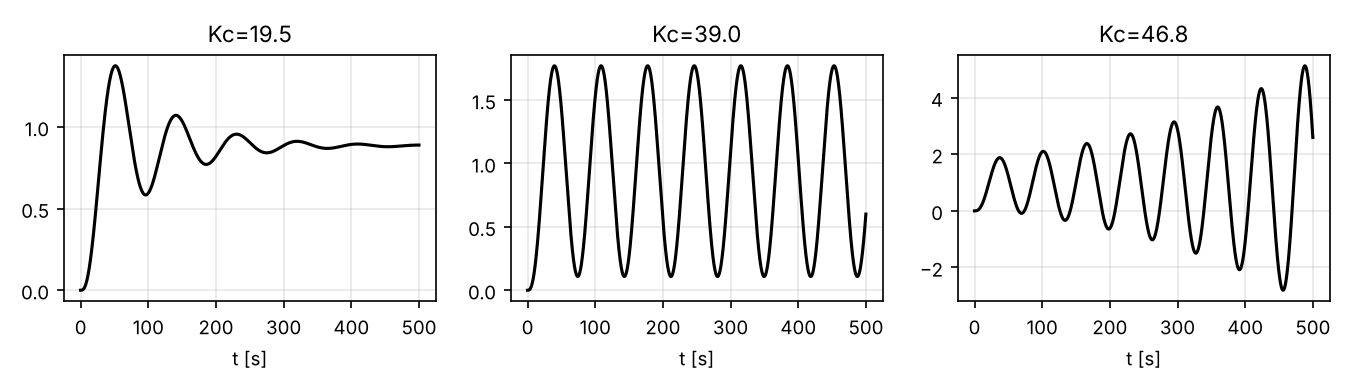
\includegraphics[width=.95\textwidth]{figs/i41_kcu.png}\caption{Teste de ganho final, simulação ideal (FT completa, controle P puro): com $0{,}5K_{cu}$ a oscilação amortece; com $K_{cu}$ é sustentada com período $T_u=68{,}85$ s; com $1{,}2K_{cu}$ cresce.}\end{figure}
\begin{center}\small
\begin{tabular}{lcc}\toprule & Previsão (FT completa) & \textbf{Experimento}\\\midrule
$K_{cu}$ & 38,97 (FOPDT daria 13,7) & \underline{\hspace{1.6cm}}\\
$T_u$ [s] & 68,85 (FOPDT daria 92,7) & \underline{\hspace{1.6cm}}\\
Amplitude da VP em $K_{cu}$ (degrau de 1 ponto) & $\approx0{,}9$ ponto & \underline{\hspace{1.6cm}}\\\bottomrule\end{tabular}\end{center}
\begin{just}Usa-se a FT \emph{completa} (e não a FOPDT) porque o Z--N exige o comportamento real no limite de estabilidade: a FOPDT subestima $K_{cu}$ em $\approx65\,\%$ (Seção 6.2). Valores medidos costumam diferir 5--15\,\% da previsão (ganho real, atraso do ciclo do PLC, quantização).\end{just}
\subsection{Parte 2: PID de Ziegler--Nichols}
Recalcular com os \emph{seus} $K_{cu}$ e $T_u$: $K_p=0{,}735K_{cu}$, $T_i=0{,}625T_u$, $T_d=0{,}1T_u$, $K_i=K_p/T_i$, $K_d=K_pT_d$. Com os valores previstos: $K_p=28{,}65$; $T_i=43{,}03$ s; $T_d=6{,}885$ s; \textbf{\texttt{kp := 28.65; ki := 0.6659; kd := 197.3; alfa := 1.0}}.
\textbf{Degrau:} como o SC pode saturar com este ganho, simulei o PID de Z--N na planta completa com os limites do programa para três pontos de operação:
\begin{center}\small\begin{tabular}{lcccc}\toprule Degrau de SP & SC mínimo & SC máximo & sobressinal & situação\\\midrule
$10\to12\,\%$ & 10,0 (satura; sem limite seria 5,5) & 86,1 & 65\,\% & \textbf{satura no limite inferior}\\
$15\to17\,\%$ & 13,6 & 98,7 & 64\,\% & no limite superior\\
$20\to22\,\%$ & 31,9 & 99,9 (sem limite: 108) & 45\,\% & \textbf{satura no superior}\\
$20\to21\,\%$ & 38,6 & 81,1 & 64\,\% & \textbf{não satura}\\\bottomrule\end{tabular}\end{center}
\textbf{Recomendação: $20\to21\,\%$} (o mesmo ponto de operação do teste de ganho final). O degrau de $10\to12$ usado na Seção~\ref{it41} (simulação sem os limites do programa) satura o SC em 10\,\%.
\subsection{Previsão da simulação ideal e planilha}
\begin{figure}[H]\centering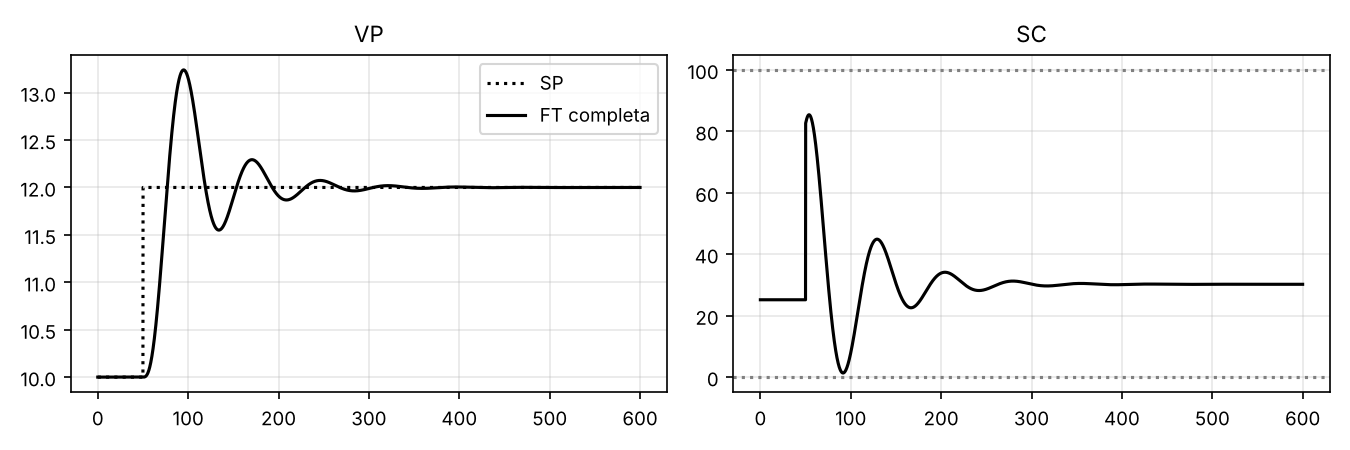
\includegraphics[width=.98\textwidth]{figs/i41.png}\caption{Item 4.1, simulação ideal (FT completa, degrau $10\to12$, sem os limites do programa): sobressinal $\approx62\,\%$ e razão de decaimento $\approx1/4$.}\end{figure}
\begin{center}\small
\begin{tabular}{lcc}\toprule Métrica (degrau $20\to21$, FT completa, com limites do programa) & Ideal & \textbf{Experimento}\\\midrule
Sobressinal [\%] & 64 & \underline{\hspace{1.6cm}}\\
$t_{63,2}$ [s] & 21 & \underline{\hspace{1.6cm}}\\
Tempo de acomodação ($\pm2\,\%$) [s] & 240 & \underline{\hspace{1.6cm}}\\
Razão de decaimento (2º pico/1º pico) & 0,24 ($\approx1/4$) & \underline{\hspace{1.6cm}}\\
SC: mínimo / máximo / final [\%] & 38,6 / 81,1 / 53,5 & \underline{\hspace{1.6cm}}\\
Salto do SC em $t=50$ s [pontos] & $K_p\Delta SP=28{,}7$ & \underline{\hspace{1.6cm}}\\
Margens da malha aberta (FT completa) & $GM=7{,}8$; $PM=22^\circ$ & ---\\\bottomrule\end{tabular}\end{center}
\begin{figure}[H]\centering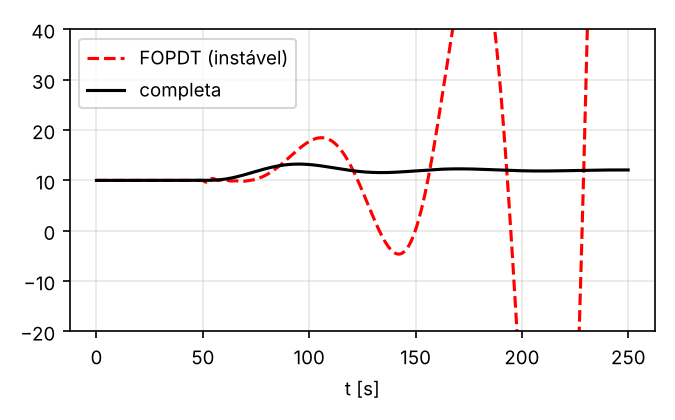
\includegraphics[width=.5\textwidth]{figs/i41_unst.png}\caption{O mesmo PID aplicado à FOPDT (instável) e à FT completa: por isso o item 4.1 só é simulado com a planta completa.}\end{figure}
\subsection{Roteiro de interpretação}
\begin{itemize}
\item \textbf{Razão de decaimento:} meça o 1º e o 2º picos acima do SP final (excesso); a razão esperada é $\approx0{,}24$. O método ``\emph{falha}'' se a razão ficar muito diferente de $1/4$ (por exemplo, por $K_{cu}$ e $T_u$ mal medidos).
\item \textbf{Sobressinal grande ($\approx64\,\%$)} é característico da razão 1/4 e da margem de fase baixa ($22^\circ$).
\item \textbf{Por que não simular com a FOPDT:} os polos de malha fechada ficam no semiplano direito ($+0{,}027\pm0{,}087j$): é instável.
\item \textbf{Ruído:} $k_d=197{,}3$ é o caso mais crítico do programa original (pico de 385 pontos por LSB). Na simulação fiel ao PLC, o programa original daria sobressinal de 82\,\% em vez de 62--64\,\% (Seção~\ref{progcorr}). Use o programa corrigido.
\end{itemize}
\begin{todo}(1) Teste de ganho final: anotar $K_{cu}$ e $T_u$ medidos. (2) Recalcular $K_p$, $K_i$, $K_d$ e digitar. (3) Degrau $20\to21\,\%$; gravar. (4) Preencher a tabela e comparar VP e SC com a simulação. Resultados: \underline{\hspace{6cm}}\end{todo}

%------------------------------------------------------------------
\section{Item 4.2 (Questão 4): I\_PD com a sintonia do 4.1}\label{q42exp}
\subsection{Objetivo e teoria}
``Aproveite a sintonia do PID para realizar um I\_PD, e explique o que acontece.'' No I\_PD, \textbf{só o integrador atua sobre o erro}; o proporcional e o derivativo atuam sobre a \emph{VP}:
\[
U(s)=\frac{K_i}{s}\big(R-Y\big)-\Big(K_p+D(s)\Big)Y,\qquad D(s)=\frac{K_d\,s}{\mu T_ds+1}\ \ (\text{no programa: derivada de 4 pontos}).
\]
Como $Y=GU$, isolando $U$ e $Y$:
\[
\frac{Y}{R}=\frac{\dfrac{K_i}{s}\,G}{1+(PI+D)\,G},\qquad\frac{U}{R}=\frac{\dfrac{K_i}{s}}{1+(PI+D)\,G},\qquad PI=K_p+\frac{K_i}{s}.
\]
Comparando com o PI\_D ($Y/R=\frac{PI\,G}{1+(PI+D)G}$):
\begin{itemize}
\item \textbf{O denominador é o mesmo} $\Rightarrow$ os mesmos polos de malha fechada (mesma estabilidade e a mesma resposta a \emph{distúrbio}, $VP/D=\frac{G}{1+(PI+D)G}$).
\item \textbf{O numerador muda:} de $(K_ps+K_i)/s$ para $K_i/s$: \textbf{o zero do PI desaparece}. O zero do PI é o responsável pelo ``chute'' proporcional ($\Delta SC(0^+)=K_p\Delta SP$) e por grande parte do sobressinal.
\item \textbf{Valor inicial:} $\Delta SC(0^+)=0$ (o SC não tem salto no degrau de SP) e o SC cresce só pela integral.
\end{itemize}
\textbf{No programa:} \texttt{alfa := 0.0}. Com $\mathtt{alfa}=0$, a \texttt{FF2GL} acumula $K_p\Delta SP$ e é subtraída de $u$, cancelando o proporcional sobre o SP (peso $b=\mathtt{alfa}=0$, Seção~\ref{alfaplc}); a integral continua sobre o erro completo e a derivada, sobre a VP.
\subsection{Como digitar e procedimento}
Mesmos parâmetros do 4.1 (com os $K_{cu}$ e $T_u$ medidos): \texttt{kp := 28.65; ki := 0.6659; kd := 197.3; \textbf{alfa := 0.0}}. Procedimento do roteiro comum (Seção~\ref{roteirocomum}), degrau $20\to22\,\%$ (o I\_PD não tem salto de SC, então o limite de 100\,\% não é problema). Se houver tempo, sobrepor com o ensaio PI\_D do 4.1.
\subsection{Previsão da simulação ideal}
\begin{figure}[H]\centering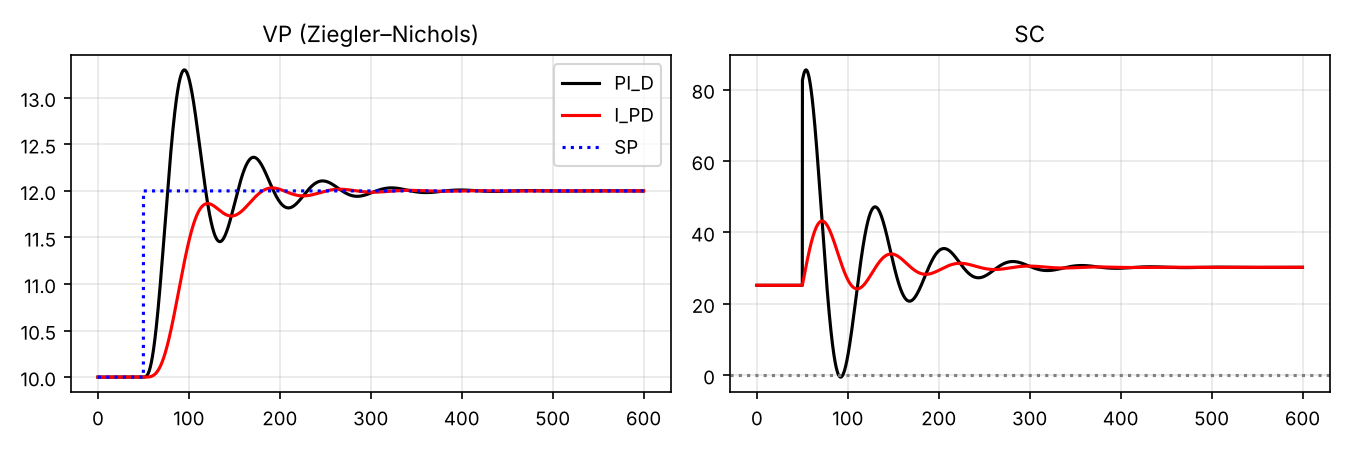
\includegraphics[width=.98\textwidth]{figs/g42.png}\caption{Item 4.2, simulação ideal (FT completa): PI\_D (preto) e I\_PD (vermelho) com a sintonia de Z--N, degrau $10\to12\,\%$.}\end{figure}
\begin{center}\small
\begin{tabular}{lccc}\toprule Métrica (FT completa, Z--N, com limites do programa) & PI\_D (4.1) & I\_PD ideal & \textbf{I\_PD experimento}\\\midrule
Sobressinal [\%] & 64--65 & 1,2 & \underline{\hspace{1.4cm}}\\
$t_{63,2}$ [s] & 21 & 46 & \underline{\hspace{1.4cm}}\\
Tempo de acomodação ($\pm2\,\%$) [s] & 210--240 & 183 & \underline{\hspace{1.4cm}}\\
Salto do SC em $t=50$ s [pontos] & $+28{,}7$ ($K_p\Delta SP$, 1 ponto) & \textbf{0} & \underline{\hspace{1.4cm}}\\
SC ($20\to22$): mínimo / máximo [\%] & 31,9 / 99,9 (satura) & 50,3 / 68,9 & \underline{\hspace{1.4cm}}\\\bottomrule\end{tabular}\end{center}
Para a sintonia de Dahlin (item 1.1) com I\_PD (degrau $20\to30$): sobressinal 0\,\%, $t_{63}=164$ s (contra 70 s do PI\_D), tempo de acomodação 434 s, SC máximo 76,2\,\% (sem pico: o SC sobe monotonicamente ao valor final, contra o pico de 88,6\,\% do PI\_D). Com a sintonia IAE do 3.1, o I\_PD (degrau $20\to25$) dá 0\,\% de sobressinal e $t_{63}=151$ s, contra 44 s do PI\_D.
\subsection{Roteiro de interpretação (``explique o que acontece'')}
\begin{enumerate}
\item \textbf{Menor sobressinal e SC suave:} o I\_PD elimina o zero do PI e o salto proporcional; a VP sobe sem o ``chute'' inicial.
\item \textbf{Mais lento:} sem a ação proporcional ``antecipada'' no SP, $t_{63}$ passa de 21 para 46 s (Z--N). Isso é o preço da suavidade.
\item \textbf{Mesma estabilidade e mesma rejeição de distúrbio:} o denominador não mudou ($PM=22^\circ$ e $GM=7{,}8$ iguais). Um distúrbio ($R_p$) teria a mesma resposta nos dois casos.
\item \textbf{Quando usar:} com ganho alto e atuador sensível a degraus de SP, ou para evitar saturação em mudanças de SP (a Tabela mostra o PI\_D saturando em $20\to22$, o I\_PD não).
\item \textbf{Relação com o 2GL:} I\_PD é o caso $b=0$ ($\mathtt{alfa}=0$); PI\_D, $b=1$ ($\mathtt{alfa}=1$); os valores intermediários são o PID 2GL do item 2.1.
\end{enumerate}
\begin{todo}Executar o I\_PD com \texttt{alfa := 0.0} (mesmos \texttt{kp}, \texttt{ki}, \texttt{kd} do 4.1) e preencher a tabela. Conferir: salto de SC $\approx0$; sobressinal $\lesssim2\,\%$; $t_{63}\approx46$ s. Comparar com o ensaio PI\_D do 4.1. Resultados: \underline{\hspace{6cm}}\end{todo}

%------------------------------------------------------------------
\section{Quadro dos ensaios}\label{quadro}
\begin{center}\small
\resizebox{\textwidth}{!}{\begin{tabular}{llllll}\toprule Item & Programa/parâmetros & Degrau & Previsão ideal & Experimento & Seção\\\midrule
1.1 & \texttt{kp 3.523; ki 0.03872; kd 39.16; alfa 1} & $19{,}5\to30$ & $t_{63}=70$ s; 0\,\% & realizado (Q11) & \ref{expq11}\\
1.2 & idem, sem VP-tracking & $SP\ne VP$ & salto $=K_p(SP-VP)$ & realizado (Q12) & \ref{expq12}\\
1.3 & idem, sem/com \texttt{STOP\_INTGR} & $25\to55\to20$ & saída da sat.\ $\approx$ 330 s / 0 & realizado (Q13a, b) & \ref{expq13}\\
2.1 & \texttt{kp 5.057; ki 0.05558; kd 56.21; alfa 0.36} & $20\to30$ & $t_{63}=104$ s; 0\,\% & \textbf{a realizar} & \ref{it21}\\
2.2 & idem, com $R_p=133{,}6$ k$\Omega$ & distúrbio & queda 2,6 pt; 134 s & \textbf{a realizar} & ---\\
3.1 & \texttt{kp 7.222; ki 0.06449; kd 71.63; alfa 1} & $20\to25$ & 2,6\,\%; $t_{63}=44$ s & \textbf{a realizar} & \ref{q31exp}\\
4.1 & ganho final; depois \texttt{kp 28.65; ki 0.6659; kd 197.3} & $20\to21$ & 64\,\%; $t_{63}=21$ s & \textbf{a realizar} & \ref{q41exp}\\
4.2 & idem 4.1, \texttt{alfa 0} & $20\to22$ & 1,2\,\%; $t_{63}=46$ s & \textbf{a realizar} & \ref{q42exp}\\\bottomrule\end{tabular}}\end{center}
